\documentclass{article}
\usepackage[utf8]{inputenc}
\usepackage{csquotes}
\usepackage[textsize=footnotesize]{todonotes}
\usepackage{subcaption}
% \usepackage{url}
\PassOptionsToPackage{hyphens}{url}\usepackage{hyperref}


\urlstyle{same}

\setlength{\parindent}{0pt}

\begin{document}

Dear Reviewer,

\vspace{0.25in}

Thank you for considering our manuscript for publication and for providing constructive feedback.
Hereunder you will find our detailed replies to all Your comments.
The changes are highlighted in the output of the latexdiff file attached to this cover letter.


\paragraph{Issue 1:}
\begin{displayquote}
"Since, one of the study aim was to reduce the data, therefore, by analysing ECG signals visually and by experiments we set the threshold of 2 which means all the data points associated with frequency more than two i.e., high QRS peaks (downward in lead V1) will be discard because the signals can classify through the base patterns." What can be understood that all frequency components above 2 are reduced to 0. However, the authors do not specify whether they mean 2 Hz (the unit is important). In this part of the paper there is no reference to the frequency band that the ECG signal covers. In the situation, as presented by the authors, then above a frequency of 2 Hz there are no longer any components derived from the ECG signal, as can be seen in the spectrograms. There are also reservations about the spectrograms presented, which have neither a time axis nor a frequency axis let alone the values that would be presented.
\end{displayquote}


\paragraph{Issue 1a:}
\begin{displayquote}
What can be understood that all frequency components above 2 are reduced to 0. However, the authors do not specify whether they mean 2 Hz (the unit is important). In this part of the paper there is no reference to the frequency band that the ECG signal covers.
\end{displayquote}

\paragraph{Answer:}
Thank you for this issue. In frequency filtration, our aim was to reduce the sample size as much as possible. Since, the Anteroseptal Myocardial Infarction can be distinguised through ST elevation in lead V1 [], therefore, we took the cutoff of high frequency component only i.e., above than 2 Hz as shown in fig. 3(a) where one can see there are two components above this cutoff. 

With regards to frequency bands, there are no such information at the PTB-XL dataset repo page except that there dataset were calculated in 500 Hz and 100 Hz sampling frequency. So, we utilized 100 Hz dataset which is mentioned in the article text i.e., Methodology section. 

\paragraph{Issue 1b:}
\begin{displayquote}
In the situation, as presented by the authors, then above a frequency of 2 Hz there are no longer any components derived from the ECG signal, as can be seen in the spectrograms. There are also reservations about the spectrograms presented, which have neither a time axis nor a frequency axis let alone the values that would be presented
\end{displayquote}

\paragraph{Answer:}
Thanks for raising this issue. Time and Frequency axis are now added into the spectrograms (as given in below fig). One can see, in the spectrogram (b), there are no frequency components above 2 Hz frequency at the Y-axis. 

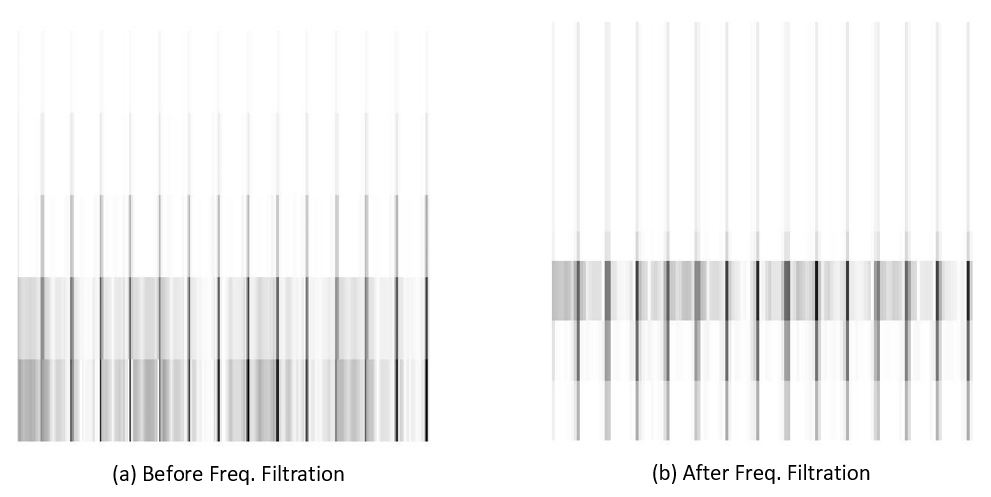
\includegraphics[scale=0.55]{before and after spectrogram.JPG}


\paragraph{Issue 2:}
\begin{displayquote}
Nor has it been explained what is the relationship of the threshold of 2 that high QRS peaks (downward in the V1 lead) will be rejected. One may ask what does frequency have to do with the amplitude of the QRS complex in the ECG signal? Improper filtering can reduce the amplitude of the QRS complex, leading to the loss of important diagnostic information.
\end{displayquote}

\paragraph{Answer:}
Thank you for this issue. As mentioned before, we were aimed to reduce the high peaks from the V1 lead becuase both of the classes can be distinguish without QRS peaks as ST elevation can be used to detect disease from Lead V1. Therefore, by visualizing the spectrograms (before filtration), we found that 2 Hz is best option because there are few component exists above this cutoff and it also do not disturb the ST elevation shape in ECG signals. 

\paragraph{Issue 3:}
\begin{displayquote}
The explanations provided in the above-mentioned issues of reducing interference in the ECG signal cannot be accepted and affect the overall perception of the submitted work for review. I suggest reading the frequency characteristics of the ECG signal, for example, as presented in the book by Clifford Gari D, Azuaje Francisco, McSharry Patrick E, Eds: ``Advanced Methods `\&' Tools for ECG Data Analysis''.
\end{displayquote}

\paragraph{Answer:}
Thank you for the issue. In the two articles referenced as [54] and [55] in the reference section of submitted paper, experiments taken by the authors and they support the wavelet transformation as a suitable method for reducing interference / signal analysis. Therefore, we beleive that WT is suitable for our work which is shown in accuracy obtained as a results.

\paragraph{Issue 4:}
\begin{displayquote}
Figure 2b,d and 3 present obtained spectrograms. In the cited paper [45] (Kang M, Shin S, Jung J, Kim YT. Classification of Mental Stress Using CNN-LSTM Algorithms with Electrocardiogram Signals. 564 Journal of Healthcare Engineering. 2021 Jun 7;2021:e9951905. Available from: https://www.hindawi.com/journals/jhe/2021/9951905/) also used spectrograms however these spectrograms are in color with the axes described. Why were the color spectrograms not obtained (presented) in the reviewed paper? 
\end{displayquote}.

\paragraph{Answer:}
Thank you for this issue. Color mapping can be changed, it only need to change cmap but according to our neural network architecture, we are passing a particular specified channel due to which we achieved higher accuracy with our proposed architecture. Additionally, the images are not in particular (or binarized), it represents several intensities or band maps based on gray color intensity. This color mapping is only for visualization purposes but in our case, it is specified as per performance of our neural network achitecture. 

\paragraph{Issue 5:}
\begin{displayquote}
Issue 8b from the previous review. I maintain that up-sampling the signal does not make sense, this part of the work I would skip.
\end{displayquote}.

\paragraph{Answer:}
Thank you for this issue. 
We agree that up-sampling gives lower accuracy than original signal.
In our investigation we checked if interpolation is able to make our analysis better.

(a) We skipped the up-sampling from Fig. 8.

We added the following text:

'We checked if interpolation (up-sampling) is able to make our analysis better. For 200Hz we get XXX accuracy, for 400Hz we get YYY accuracy,
therefore '.

From Figure 6, it can be seen that the highest accuracy is achieved just for the sampling frequency of 100 Hz? Any other frequency means a decrease in accuracy, because where to get additional information about the signal, when physically this information is not there. The results achieved are just the result of interpolation. Such a study would make sense if the original sampling frequency of the ECG signal was high enough, such as 1 kHz or 2kHz. Another issue is connecting the points on the graph with 6 straight lines, after all, no calculations were made for 159 Hz.


\vspace{0.25in}

Sincerely yours,\\
Muhammad Farhan Safdar\\
for the authors

\end{document}
